%
%
%
%\VignetteIndexEntry{An R package for visualization and analysis of Cufflinks high-throughput sequencing data}
%\VignetteKeywords{cummeRbund,visualization,sequencing,cufflinks}
%\VignettePackage{cummeRbund}
%
%%%%%%%%%%%%%%%%%%%%%%%%%%%%%%%%%%%%%%%%%%%%%%%%%%%%%%%%%%%%%%%%%%%%%%%%%%%
\documentclass[10pt]{article}
\usepackage{amsmath}
\usepackage[authoryear,round]{natbib}
\usepackage{hyperref}
\hypersetup{
    colorlinks,
    citecolor=black,
    filecolor=black,
    linkcolor=red,
    urlcolor=black
}
\usepackage{theorem}
\usepackage{float}
\usepackage{ifthen}
\usepackage[OT1]{fontenc}

\newcommand{\R}{{\textsf{R}}}
\newcommand{\code}[1]{{\texttt{#1}}}
\newcommand{\term}[1]{{\emph{#1}}}
\newcommand{\Rpackage}[1]{\textsf{#1}}
\newcommand{\Rfunction}[1]{\texttt{#1}}
\newcommand{\Robject}[1]{\texttt{#1}}
\newcommand{\Rclass}[1]{{\textit{#1}}}
\newcommand{\Rmethod}[1]{{\textit{#1}}}
\newcommand{\Rfunarg}[1]{{\textit{#1}}}

\bibliographystyle{plainnat}
\title{cummeRbund: Visualization and Exploration of Cufflinks High-throughput Sequencing Data}

\author{Loyal A. Goff, Cole Trapnell}
\date{1 April, 2011}

\usepackage{Sweave}
\begin{document}


\maketitle

\tableofcontents

\section{Introduction}
	\Rpackage{cummeRbund} is a visualization package for Cufflinks high-throughput sequencing data. The base class, \Rclass{cuffSet} 
	is a 'pointer' to cufflinks data that are stored out-of-memory in a sqlite database.
	
\section{CummeRbund Classes}

\subsection{CuffSet Class}

\subsection{CuffData Class}

\subsection{CuffFeatureSet Class}

\subsection{CuffFeature Class}
	
\section{Reading cuffdiff output}
\begin{Schunk}
\begin{Sinput}
> cuff <- readCufflinks(dir = fileDir)
> cuff
\end{Sinput}
\begin{Soutput}
CuffSet instance with:
	 3 samples
	 35695 genes
	 102603 isoforms
	 54339 TSS
	 20584 CDS
\end{Soutput}
\end{Schunk}

\subsection{Reading additional annotation files}


\section{Global statistics}
Several plotting methods are available that allow for quality-control or global analysis of cufflinks data. For example, to assess the
distributions of FPKM scores across samples, you can use the \Rmethod{csDensity} plot (Figure 1).
\begin{Schunk}
\begin{Sinput}
> dens <- csDensity(cuff@genes)
\end{Sinput}
\end{Schunk}

\begin{figure}[ht]
\begin{center}
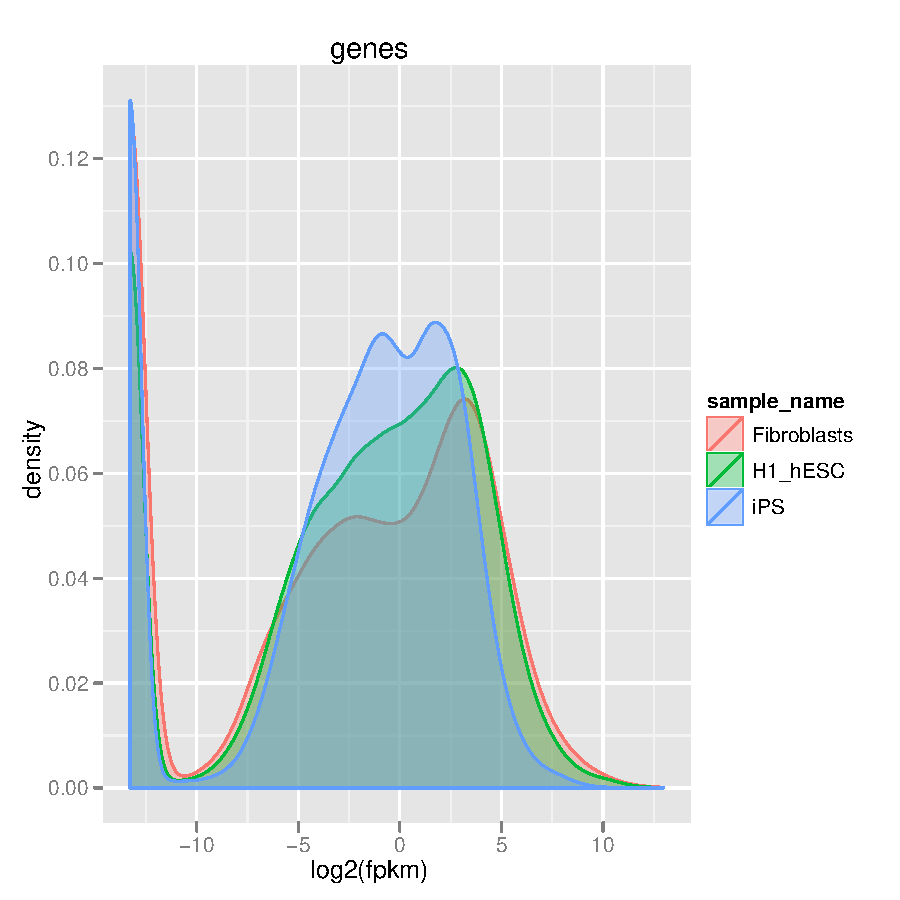
\includegraphics{cummeRbund-manual-global_plots_dens}

\end{center}
\caption{Density plot per sample of cufflinks output FPKM values.}
\end{figure}

Boxplots can be visualized using the \Rmethod{csBoxplot} method (Figure 2).
\begin{Schunk}
\begin{Sinput}
> b <- csBoxplot(cuff@genes)
\end{Sinput}
\end{Schunk}

\begin{figure}[ht]
\begin{center}
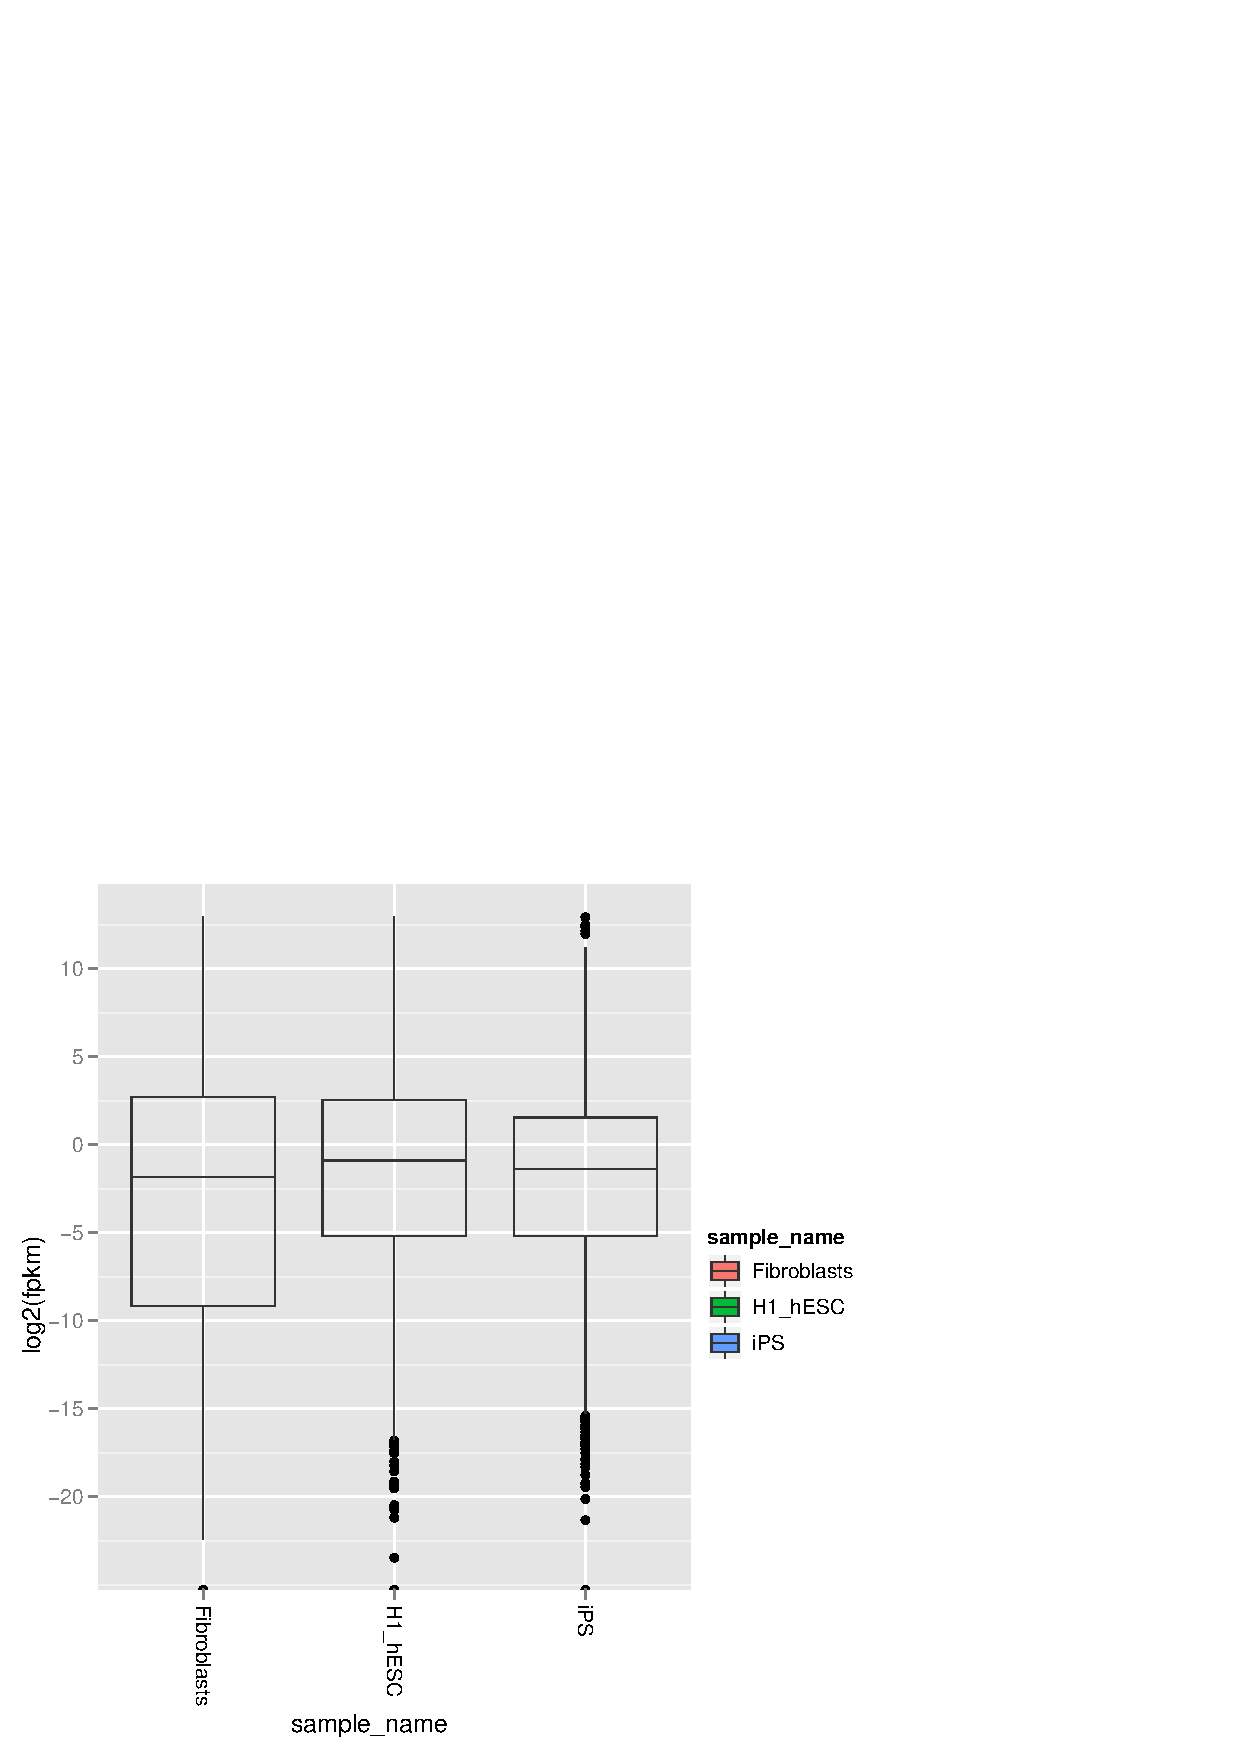
\includegraphics{cummeRbund-manual-global_plots_box}

\end{center}
\caption{Box plot of FPKM values from cufflinks output.}
\end{figure}

Pairwise comparisons can be made by using \Rmethod{csScatter} (Figure 3). You must specify the sample names to use for the $x$ and $y$ axes:
\begin{Schunk}
\begin{Sinput}
> s <- csScatter(cuff@genes, "H1_hESC", "Fibroblasts", 
+     smooth = T)
\end{Sinput}
\end{Schunk}

\begin{figure}[ht]
\begin{center}
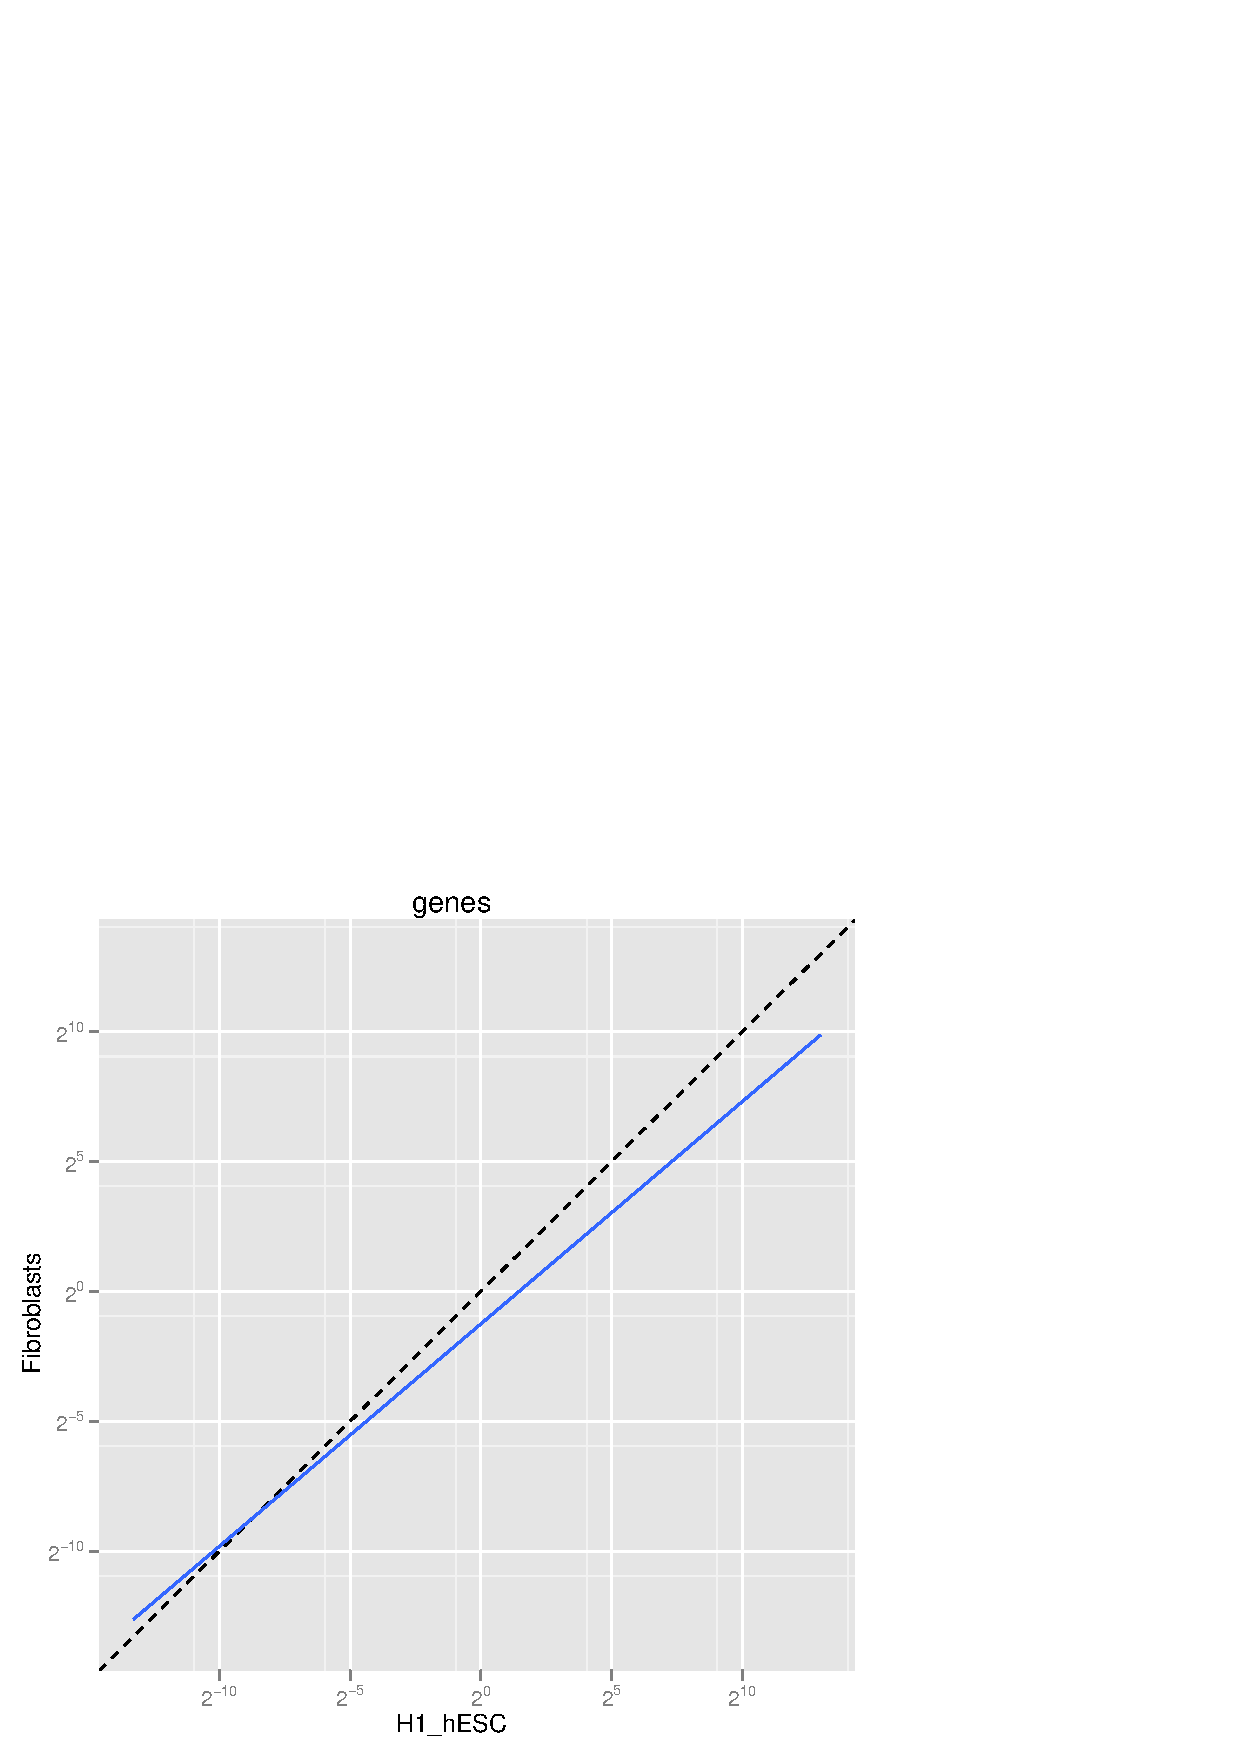
\includegraphics{cummeRbund-manual-global_plots_scatter}

\end{center}
\caption{Scatter plot comparing the FPKM values of two samples from cufflinks output.}
\end{figure}

Volcano plots are also available for the \Rclass{CuffData} objects. Again, you must specify the comparisons by sample_name.
\begin{Schunk}
\begin{Sinput}
> v <- csVolcano(cuff@genes, "H1_hESC", "Fibroblasts")
\end{Sinput}
\end{Schunk}

\begin{figure}[ht]
\begin{center}
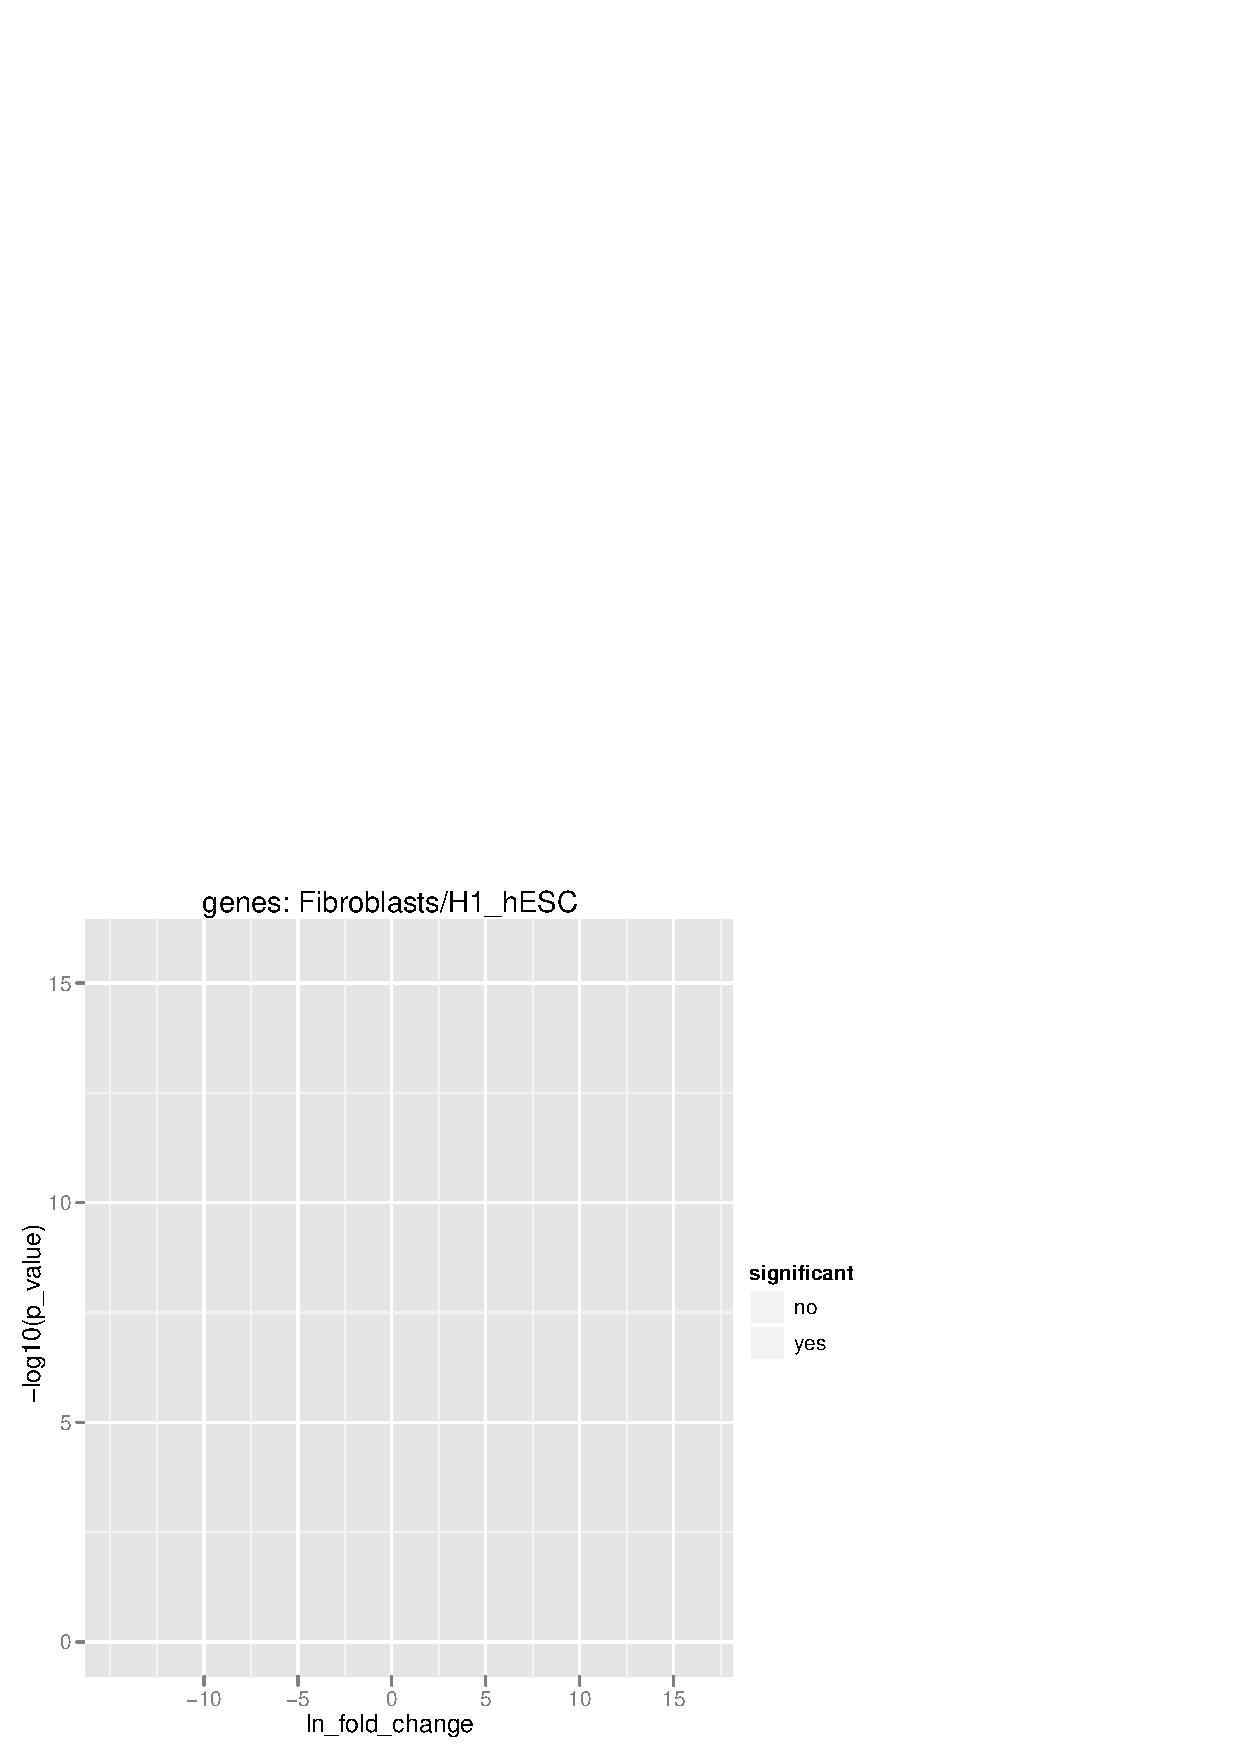
\includegraphics{cummeRbund-manual-global_plots_volcano}

\end{center}
\caption{Volcano plot of ln fold change vs significance.}
\end{figure}

\clearpage

\section{Creating Gene Sets}

\subsection{Geneset level plots}

\section{Individual Genes}

\subsection{Gene-level plots}

\section{Session info}
\begin{Schunk}
\begin{Sinput}
> sessionInfo()
\end{Sinput}
\begin{Soutput}
R version 2.12.1 (2010-12-16)
Platform: x86_64-apple-darwin9.8.0/x86_64 (64-bit)

locale:
[1] C/en_US.UTF-8/C/C/en_US.UTF-8/en_US.UTF-8

attached base packages:
[1] grid      stats     graphics  grDevices utils     datasets 
[7] methods   base     

other attached packages:
[1] cummeRbund_0.1.2 ggplot2_0.8.9    proto_0.3-8     
[4] reshape_0.8.3    plyr_1.4         RSQLite_0.9-4   
[7] DBI_0.2-5       

loaded via a namespace (and not attached):
[1] digest_0.4.2 tools_2.12.1
\end{Soutput}
\end{Schunk}

\end{document}
